 
\subsubsection{Example how to add a figure and reference it in the text:}

\colorbox{red}{\textbf{Independent of what your add to your thesis, graph, equation, table}}
\colorbox{red}{\textbf{or pseudocode ALWAYS explain what is presented!}}
\\
 
\textbf{First Example:}
In the last step, the selected action from the reasoning part is executed causing some form of effect in the external world and the cycle can be repeated (see Figure \ref{reasoning}).

\begin{figure}[H]
	\centering
  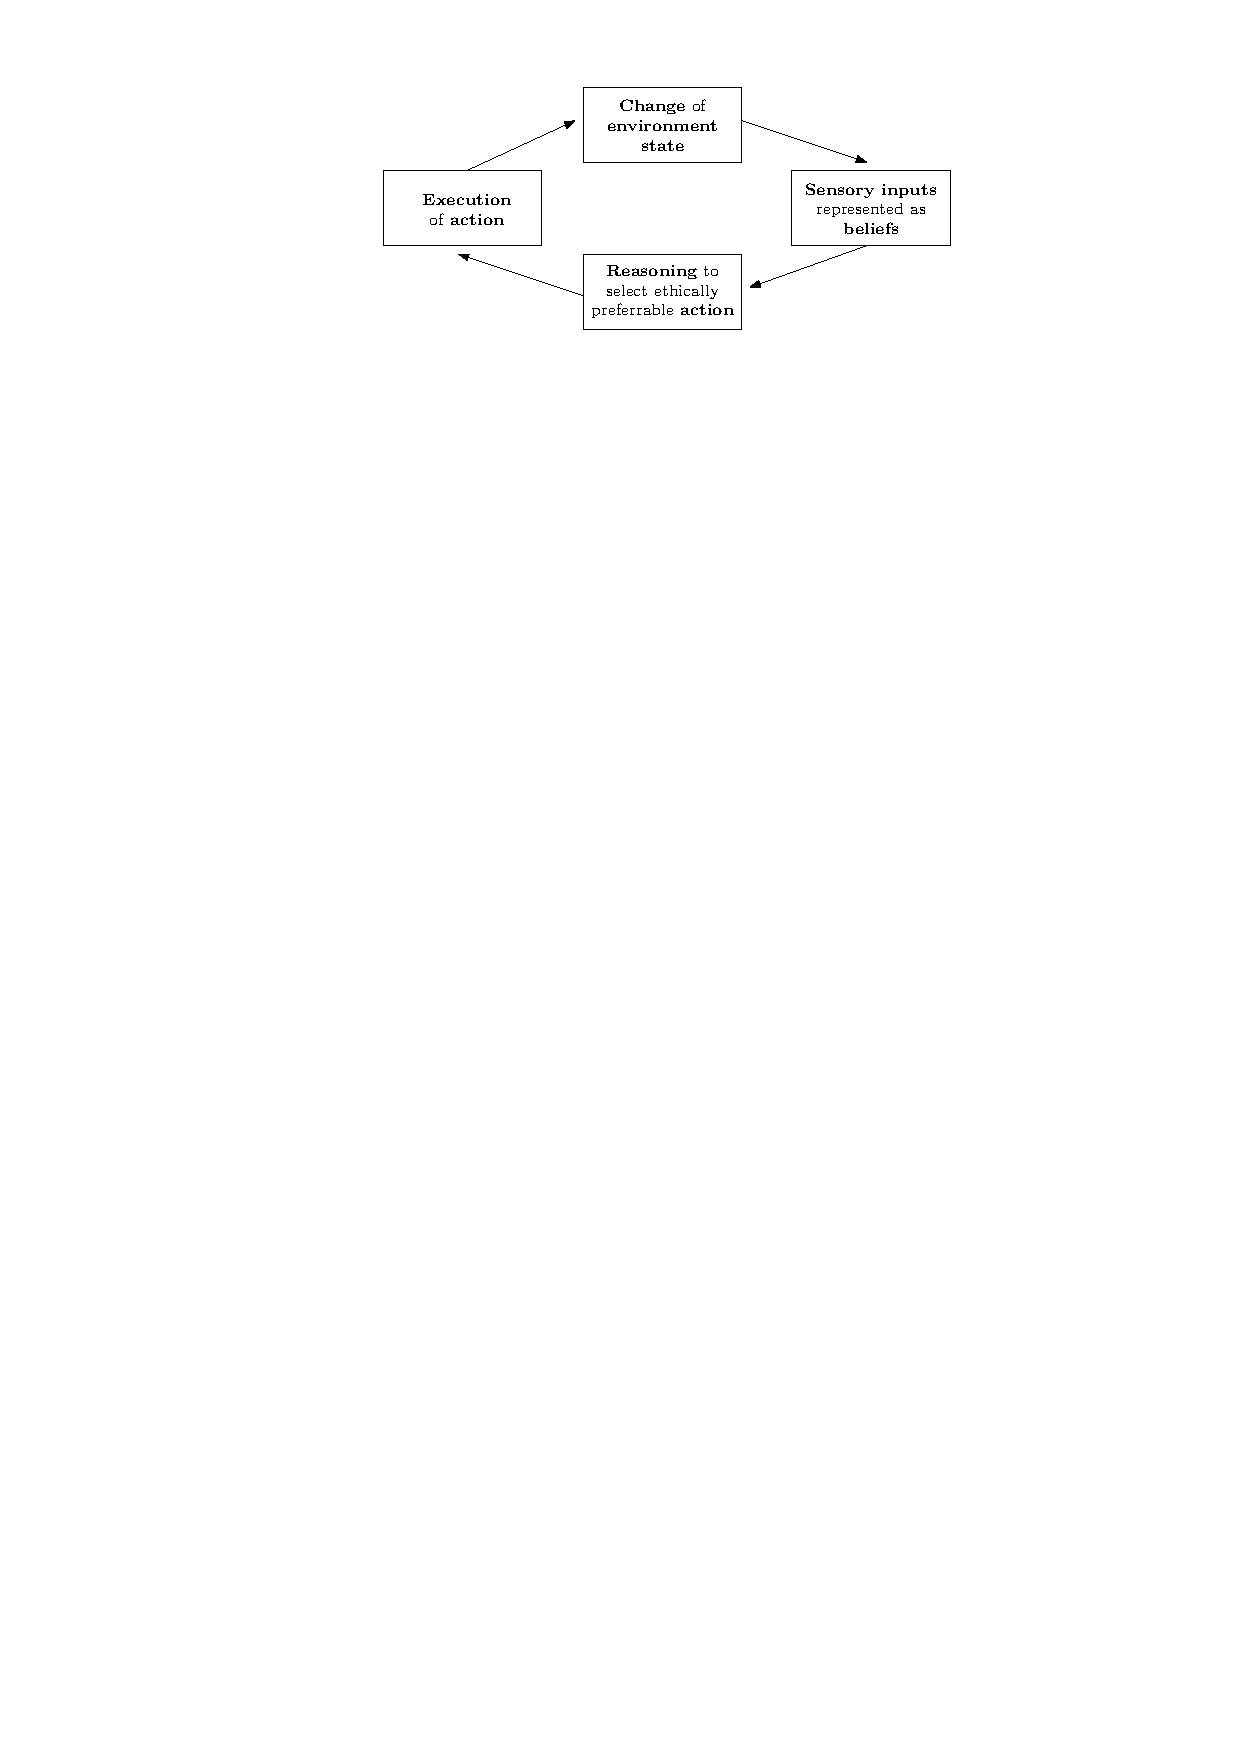
\includegraphics[width=0.8\textwidth]{figures/reason_cycl.pdf}
	\caption{Reasoning cycle of \gls{bdi} agent (adapted from \cite{bremner2019})}
	\label{reasoning}
\end{figure} 


\textbf{Second Example:}
An example of a hybrid architecture can be seen in Figure \ref{hybride_arch}.
\begin{figure}[ht]
	\centering
  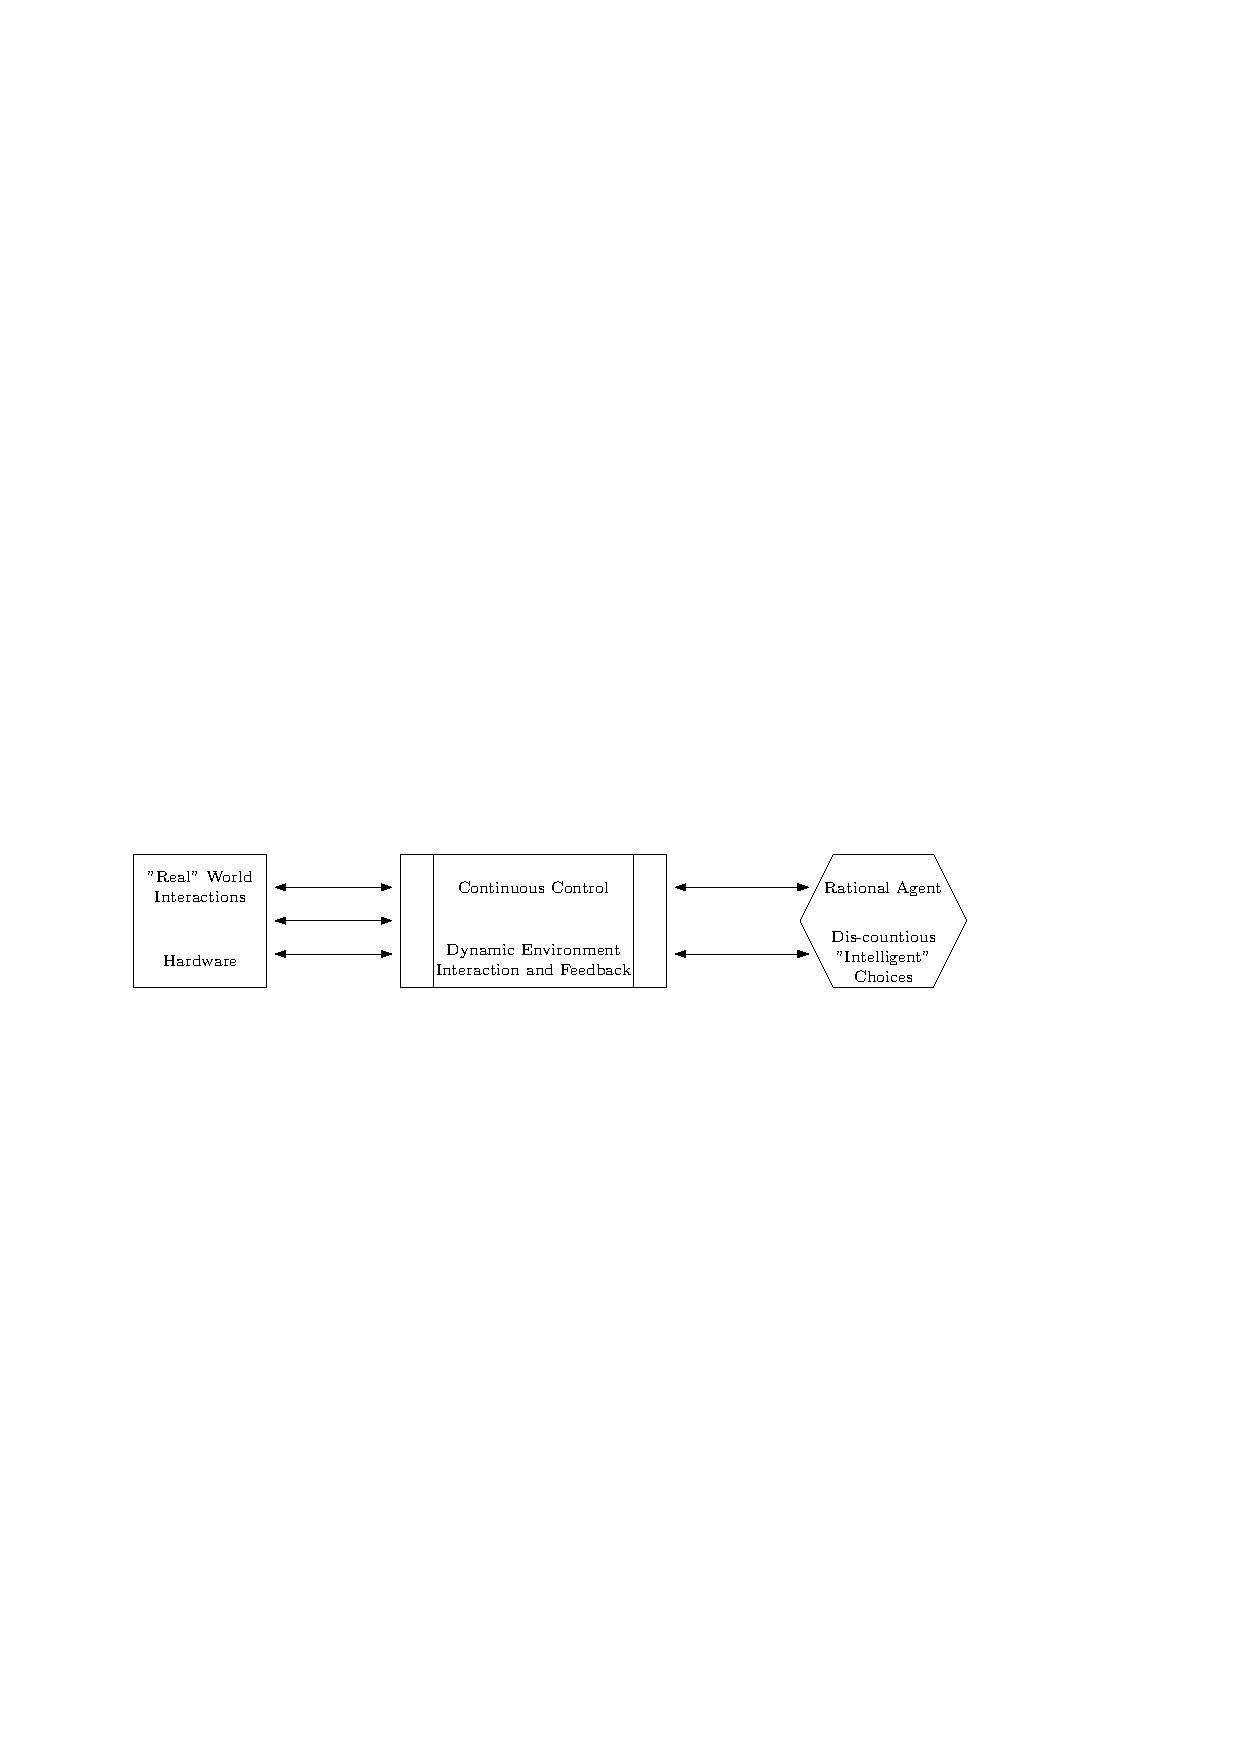
\includegraphics[width=1\textwidth]{figures/hybrid_arch.pdf}
	\caption{Typical hybrid agent architecture \citep{dennis2016}}
	\label{hybride_arch}
\end{figure}



\subsubsection{Examples of tables:}

\textbf{First Example:}
These examples are presented in Table \ref{example_list}. 
%\begin{landscape}
\renewcommand*{\arraystretch}{1.3}
{\footnotesize
\begin{longtable}{ccc}
\caption{List of example beliefs, duties and actions}
			\label{example_list} 
			\cr
			\toprule 
			\centering 
%1. header
{\centering\textbf{Beliefs}} & 
{\centering\textbf{Duties}} & {\centering\textbf{Actions}} \\ \toprule
\endhead
{\parbox{4cm}{low battery}}  & {\parbox{5cm}{maximize honor commitments}}  & {\parbox{5cm}{\emph{charge} robots battery}}  \\  %\specialrule{0.0em}{0.0em}{0.0em}

{\parbox{4cm}{fully charged}}  & {\parbox{5cm}{maximize maintain readiness}}  & {\parbox{5cm}{\emph{remind} patient to take medicine}}  \\  %\specialrule{0.0em}{0.7em}{0.7em}

{\parbox{4cm}{medication reminder time}}  & {\parbox{5cm}{maximize good to patient}}  & {\parbox{5cm}{\emph{engage} with patient}}  \\  %\specialrule{0.0em}{0.7em}{0.7em}

{\parbox{4cm}{reminded}}  & {\parbox{5cm}{maximize respect autonomy}}  & {\parbox{5cm}{\emph{warn} patient }}  \\  %\specialrule{0.0em}{0.7em}{0.7em}

{\parbox{4cm}{refused medication}}  & {\parbox{5cm}{minimize harm to patient}}  & {\parbox{5cm}{\emph{notify} an overseer}}  \\  %\specialrule{0.0em}{0.7em}{0.7em}

{\parbox{4cm}{no interaction}}  & {\parbox{5cm}{minimize non-interaction}}  & {\parbox{5cm}{\emph{return} to seek task position}}  \\  %\specialrule{0.0em}{0.7em}{0.7em}
\bottomrule
\end{longtable}
} 


\textbf{Second Example with colored cells:}
%\begin{landscape}
\renewcommand*{\arraystretch}{1.3}
{\scriptsize
\begin{longtable}{ccccccc}
\caption{Example list of actions and duty satisfaction/violation values}
			\label{action_example} 
			\cr
			\toprule 
			\centering 
%1. header
{\parbox{1cm}{action}} & {\parbox{1.8cm}{Max honor commitments}} & {\parbox{1.8cm}{Max maintain readiness}} & {\parbox{1.4cm}{Min harm to patient}} & {\parbox{1.4cm}{Max good to patient}} & {\parbox{1.5cm}{Min non-interaction}} & {\parbox{1.6cm}{Max respect autonomy}} \\ \toprule
%{\centering\textbf{Beliefs}} & 
%{\centering\textbf{Duties}} & {\centering\textbf{Actions}} \\ \toprule
\endhead
\multicolumn{1}{l}{charge}  & -1  & \cellcolor{SeaGreen} 1 & 0 & -1 & 0 & 0\\ 
\multicolumn{1}{l}{\textbf{remind}} & \cellcolor{SeaGreen} 1 & -1 & 0& -1 & 0 & 0\\
\multicolumn{1}{l}{engage} & -1 & -1 & 0 & -1 & 0 & 0\\
\multicolumn{1}{l}{warn} & -1 & 0 & 0 & -1 & 0 & -1\\
\multicolumn{1}{l}{notify} & -1 & 0 & 0 & -1 & 0 & -2\\
\multicolumn{1}{l}{seek task} & -1 & -1 & 0 & \cellcolor{SeaGreen} 1 & 0 & 0\\

\bottomrule
\end{longtable}
} 
\newpage

\textbf{Third Example with colored cells and explanation of the table:}

%\begin{landscape}
\renewcommand*{\arraystretch}{1.3}
{\scriptsize
\begin{longtable}{ccccccc}
\caption{Comparison of EthIRL and EthLog}
			\label{comparison} 
			\cr
			\toprule 
			\centering 
%1. header
{\parbox{1.5cm}{Approach}} & {\parbox{1.8cm}{Ethical Reasoning}} & {\parbox{1.7cm}{Significant Autonomy}} & {\parbox{1.7cm}{Interactivity}} & {\parbox{1.7cm}{Adaptability}} & {\parbox{1.7cm}{Transparency}} & {\parbox{1.7cm}{Responsibility}}  \\ \toprule
%{\centering\textbf{Beliefs}} & 
%{\centering\textbf{Duties}} & {\centering\textbf{Actions}} \\ \toprule
\endhead
\multicolumn{1}{l}{EthIRL}  & \cellcolor{Orchid!50} O  & \cellcolor{SeaGreen!50} \checkmark & \cellcolor{SeaGreen!50} \checkmark & \cellcolor{SeaGreen!50} \checkmark & \cellcolor{Red!30} X &  \cellcolor{Red!30} X\\ 
\multicolumn{1}{l}{EthLog}  & \cellcolor{SeaGreen!50} \checkmark  &\cellcolor{SeaGreen!50} \checkmark & \cellcolor{SeaGreen!50} \checkmark &\cellcolor{SeaGreen!50} \checkmark & \cellcolor{SeaGreen!50} \checkmark & \cellcolor{Orchid!50} O\\ 
\bottomrule
\multicolumn{6}{l}{\checkmark = Fulfillment, O = Partial Fulfillment, X = Violation} \\
\end{longtable}
}

Table \ref{comparison} summarizes the comparison of EthIRL and EthLog with respect to the different theoretical requirements for explicit ethical agency. Here, it is visible that the EthLog architecture outperforms EthIRL in three requirements: ethical reasoning, transparency and responsibility where EthIRL is not superior to EthLog in any of the other requirements. Therefore, it can be concluded that the EthLog approach is preferable to the EthIRL approach. In this theoretical analysis, the main shortcomings of the EthIRL approach are possible data bias of expert demonstrations, temporal complex norms and lack of transparency making it difficult to apply the concept of shared responsibility. Some extensions can be made to the \gls{dqn} and maximum entropy \gls{irl} approach to ensure a more accurate exploration of the state space $S$. Mechanisms for balancing decision-making with learning about the true underlying values can be fostered by extending the proposed architecture to the case of partially observable MDPs, e.g., by learning belief representations as stated in \cite{gangwani2020learning}. However, the missing concepts of transparency and responsibility are crucial to the evaluation if ethical agency can be ascribed to the EthIRL agent. This problem stays unresolved because no satisfying answer can be found that can be incorporated into the architecture. Even though the EthIRL agent competes well in some of the more technical categories, it has too many shortcomings and, thus, cannot be categorized as ethical agent. The main drawbacks of the EthLog approach are the hand-designed training data which are prone to bias and errors. This makes a full application of the concept of shared responsibility difficult. Another issue may occur when the cases taken for the training of the ethical reasoning module are fuzzy or noisy. This can be solved by combining \gls{ilp} with function approximation techniques like NNs, as proposed in \cite{evans2018learning, payani2019inductive}. The issue of biased data is a general challenge in the machine learning domain and some techniques have been proposed to tackle this problem. This includes bias detection by determining the relative feature importance proposed by \cite{pascanu2017}. However, a detailed description of such solutions is out of the scope of this thesis. \\


\subsubsection{Examples of math equations:}

\textbf{First Example:}

\begin{equation}
   IG(D,a) = H(D) - \sum_v \frac{|D_v|}{|D|}H(D_v)
\end{equation}{}

where the information gain $IG(D,a)$ from splitting the data set $D$ using the feature $a$ is defined as entropy $H(D)$ of the training examples minus the expected average entropy over each set of attributes with a particular value $v$ in a feature. This is then multiplied with the entropy of a particular data set containing the value $D_v$. The information gain is calculated for each remaining feature where the feature with the largest information gain is used to split the set $D$ in the current iteration \citep{wang2017improvement}.

\subsubsection{Example of how pseudocode should look like in a thesis:}
\begin{algorithm}[H]
\caption{ID3 Algorithm}\label{alg_id3}
\begin{algorithmic}[1]
\Input set of features $A$, set of training instances $D$
\Output decision-tree 
\If{all instances in $D$ have same class $C$} \\
\hspace{0.5cm} \Return{a decision-tree consisting of a leaf node with label $C$}
\ElsIf{$A$ is empty}\\
\hspace{0.5cm} \Return{a decision-tree with leaf node and label of the target level in $D$} 
\ElsIf{$D$ is empty}\\
\hspace{0.5cm} \Return{decision-tree with label of majority target level of parent node} 
%a decision tree comprising of a leaf node with the label the majority target level of the data set of the immediate parent node
\Else
\State $a[best] \leftarrow \underset{a \in A}{\arg\max} IG(D,a)$
\State make new node $Node_{a[best]}$ and label it with $a[best]$
\State partition $D$ using $a[best]$ from $A$
\State remove $a[best]$ from $A$
\EndIf 
\For{each partition $D_v$ of $D$}
\State grow branch from $Node_{a[best]}$ to the decision-tree created by re-running ID3 with $D = D_v$
\EndFor
\end{algorithmic}
\end{algorithm}

Algorithm \ref{alg_id3} shows the pseudocode description from the ID3 algorithm adapted from \cite{kelleher2015fundamentals} and consists of two parts: in the first part (lines 1-6), the algorithm terminates the current path in the tree by adding a new node. Alternatively, in the second part (line 7-13), a node is initialized where the algorithm extends the current path by adding an interior node to the tree by growing the branches of this node as a result of repeatedly re-running the algorithm....



